\chapter{云上世界,万物互联}
\label{cha:cloud-computing-and-iot}

\begin{intro}
  无可否认,如今的世界正在步入「云」与「智能」的时代:办公有云文档、娱乐有云游戏、科研有云计算……各色以「云」为名的服务围绕着我们,建构云上的世界;智能穿戴设备、智能家具、智能电器……各种智能设备在市场上涌现,令万物得以互联。本章,我们就来了解这一切背后的技术:云计算与物联网。看完这一章,你或许会领会这些问题的答案:
  \begin{itemize}
    \item 「云」是什么,「物联网」又是什么?
    \item 「云计算」是什么?为什么它这几年这么火?
    \item 「物联网」到底是如何应用的?它又与云计算之间有什么关系?
    \item 未来的世界会是什么样子?
  \end{itemize}
\end{intro}

「云计算」(Cloud Computing)与「物联网」(Internet of Things,简称 IoT)两个词,相信你早已耳熟能详。无论是我们日常的学习、工作和生活,还是近来新兴的「智能家居」,或者是新闻上经常听到的「互联网+」,都离不开它们二位。一言略之,云计算能为物联网提供强大的计算和存储能力,而物联网可以拓展「云」的边界,二者一同,构筑了万物互联的云上世界。如果不出意外,本章将是《你缺计课》正文的最后一章,在此尾声之际,来听一个——或者几个故事吧。

\begin{note}
  本章所有故事均为虚构,如有雷同,纯属巧合。
\end{note}

\section{引子·《你缺计课》编委会隆重会面}

今天是 2024 年的中秋,大家都在与亲朋好友共度佳节,Windy 也不例外。本打算南下拜访亲戚,但机缘巧合,他去往的是 Hans 所在的城市。机会难得,Windy 便决定顺路见一见 Hans。于是,《你缺计课》编委会为数不多的会面次数,又添一回。

沿海城市,经济发达,吸引着全国的高校在这儿设立各种「校区」和「研究生院」,Hans 所在的学校就是这样。Windy 坐上地铁,告知 Hans 自己即将来访的事情,却得到了「我先起个床」的回复。

「这就是大学生作息吗?都快要一点了!」

「反正今天没事——今天好像有点热,你就在地铁口等我吧。」

三十分钟对于地铁旅途而言算有点久了,但对起床下楼而言却有些仓促。南方沿海九月的午后,大气对流裹挟的雨水总是不期而至。Windy 望着雨幕,在地铁站出口坐了一会,终于看到了 Hans 匆忙而至的身影——以及他手中的两把伞。

「你怎么有两把伞?」

「这不是看\regcolor{您}来了吗,特地去买的!」

「?」

穿过琳琅满目的工地和山重水复的小巷,Windy 跟着 Hans 来到了他的学校。

「这儿怎么到处在建东西?」

「我们『工地大学』可不是白叫的。来参观参观我们的学校,虽然这地方有点小——毕竟这里的地寸土寸金——但是条件还是不错的!」

说话间,两人走进一栋楼,来到了一间机房外。机房里,零星有几个人坐在电脑前忙活。没想到中秋佳节时,仍是工作日。

Hans 走到一台电脑前坐下,按下电源键:「写《你缺计课》了吗?」

「别急,这不放假吗。」

「我跟你说,交不上稿,都得完。」Hans 熟练地远程到自己宿舍的电脑,打开了正在编辑的《你缺计课》,「请。」

「我是来干这个的?」Windy 和电脑面面相觑。

「也不是不行对吧,」Hans 一边说着,一边改掉了文章里的两个错别字,「我每次来机房都会用这远程桌面来操控自己的电脑,毕竟自己的电脑里软件齐活,好用。」

「你说,远程桌面算不算一种服务器?」

「或许呢,不过这种『服务器在自己这』的模式现在还是少见,不像以前……」

\section{第一幕·苦衷 2004·本地部署之痛}

千禧年交替的钟声仿佛仍在耳边回荡。2004 年,互联网的浪潮以排山倒海之势涌向这片古老的土地,机遇、梦想、金钱……无尽的可能藏在这片蓝海之下,为这片大地注入新的活力。时代潮头,总有人乘风而起。辞去安稳的工作,他带着自己数年的积蓄,投入了互联网的浪潮中。

他的目标,是在省城开一家软件公司,瞄准「办公自动化」这一领域。但在互联网初入之际,运营一家软件公司的成本显然不容小觑。为此,他四处筹款,东拼西凑,好歹是凑够了地盘与设备的钱;又四处游说,召集同伴,最终与几位志同道合的伙伴组成了最初的公司。他们雄心勃勃,斗志昂扬,准备在互联网行业大干一场。

「各位,我们的目标,是占领互联网行业的一亩三分地,然后做大、做强。大家有没有信心?」

「加油!」

此后,他们立马投入到紧锣密鼓的软件开发工作中。随着时间的推移,一套「办公一体化平台」软件初具规模。这款软件,不仅能帮助企业实现任务分配、项目进度跟踪、经费管理、材料归档等功能,更支持企业内部员工之间在线通信。小本经营的他们,选择以低廉的价格提供软件与服务,换来更大的市场份额。报纸上的广告位和自己的人脉,也成为了他们最优先的宣传渠道。靠着这些策略,他们的软件受到当地许多中小企业的青睐,订单也接踵而至。这第一桶金让整个公司都喜气洋洋,大家认为自己的努力得到了回报。

然而,经年累月的运营下,一些潜在的问题终于浮出了水面。小本经营的公司,人力、设备,就连办公室的空间都非常有限。但随着客户越来越多,他们又需要不断添置服务器来应对越来越高的访问量,空间、人力,乃至电力与网络的费用也随之上涨。如此一来,「低价」的策略,随着用户量的增加,成为了公司发展的瓶颈。他们无数次计算着公司的盈亏,他问:「我们的成本是不是又要上涨了?」

也总是有这样的回答:「对,增加服务器的费用太多了,还有随之而来的各种杂七杂八的维护费用,我们实在负担不起,除非提高我们软件的售价。」

「不行!如果提高售价,我们的客户会流失许多。」

「但这是唯一的办法了!」

「……」

四年时光说长也长,长在他们软件公司经历起起又落落;但又如弹指一挥,就像他在四年后依然是一位「打工人」。虽然公司的经营情况差强人意,但相比当初的目标仍有距离,成本供需的平衡更让他心力交瘁。大公司的产品,虽然价格更高,但用户体验、宣传力度、服务质量显然也与他们不在一个量级。最终,他与伙伴虽痛心,但不得不做出艰难抉择——停止后续开发、不再出售软件。他的软件,在国产软件的历史长河中,荡下不轻不重的一缕波纹。

\section{幕间·一}

「这就是世纪初,这个行业面临的大难题之一。」Hans 结束了故事。

「也是,网络是连接我们与远方的桥梁,服务器肯定是这里面重要的组成部分。但一台服务器的价格肯定不便宜,在互联网还不发达的时代的确是不小的麻烦。」Windy 若有所思。

「没错,\regcolor{服务器其实就是一台性能强劲的电脑,作用就是和许多其他设备频繁通信,为它们提供『服务』}。比如说《你缺计课》网页版的服务器,在你用浏览器访问《你缺计课》时,就会给你发回网页的内容。又比如微信的服务器,为许许多多微信用户提供服务,在他们互发消息时充当中间的『桥梁』来转发消息。」

\begin{figure}[htb!]
  \centering
  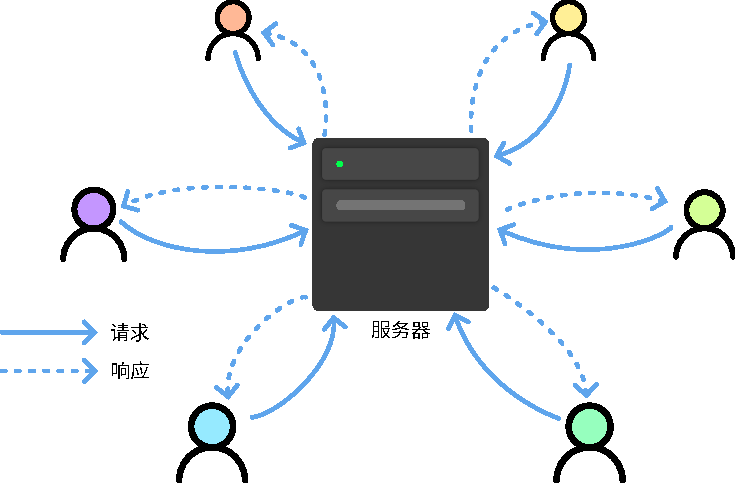
\includegraphics[width=.8\textwidth]{assets/surpass/Server_and_users.pdf}
  \caption{服务器与用户}
  \label{fig:Server_and_users}
\end{figure}

「也就是说,为了服务不掉线,服务器必须 24 小时开机咯?」Windy 随意瞥了一眼门外,只见一间挂着「高性能计算中心」牌匾的房间大门紧闭。玻璃窗内,星星点点的黄绿色光芒隐约闪烁,错落有致的一排排机器正在轰鸣。

「对。」

「那这么一来,电费也是开支大头——哦对了还有网络,既然服务器的作用是连接到其他许多电脑提供服务,那肯定需要高速、低延迟,还能直接从外面访问的网络。所以,要想搭建服务器,还得向运营商买专用宽带,这又是一笔开支。也难怪『他』做不下去了,这应该就是苦痛的根源。」

「是的。\regcolor{这种架构就是『本地部署』:服务器位于每个组织的本地,由组织自己管理。}但是很显然,这种模式让那些小微企业难以负担,将无数想进军互联网行业的人挡在了门外。」

「诶,『本地部署』这个词我好像也在好多\hyperref[cha:bring-intelligence-to-machines]{\CJKunderwave{讨论 AI 的文章}}里都看到过,它们是同一个『本地部署』吗?」

「其实它们是完全相同的意思,只不过『本地』相对的对象不一样。在介绍 AI 时,『本地』指的就是用户;而在刚刚我们的例子中,『本地』则指组织自己——这栋楼没什么好看的了,我们去别的地方看看。」

「你不饿吗?现在都快两点了,我是吃了早茶\footnote{「吃早茶」是一种广东民间的饮食风俗,一般在早晨或临近中午时以茶配点心与亲朋好友相聚。}过来的。」

「你说得对,那不如找个地方吃饭。」

对流的雨水来得快去得也快,就这么一下,天空已晴空万里。这个时候,学校里的食堂大都已经午休,大叔与大妈们躺在长座椅上,缓解中午带来的劳累。两人来到一家餐馆——不过,明亮的灯光、精致的桌椅和超大的落地窗让这里看起来更像卖漂亮甜品的咖啡馆。

落座后,两人点了一份牛排与一份炸鱼,附赠两杯饮料。大快朵颐间,他们仍不忘刚才的话题。Windy 问:「那既然买服务器很多人都负担不起,有没有别的商业模式呢?」

Hans 咽下一块牛排:「有的。后来人们想让许多这种『位于网络另一端』的服务器集中在一起,\regcolor{变『买』为『租』},按需出租给有需要的人,这样成本就可以下降许多。」

「确实,这有点像天上的云,大地之上的人都能看到他们,云也能给这片大地『雨露均沾』。」

\begin{figure}[htb!]
  \centering
  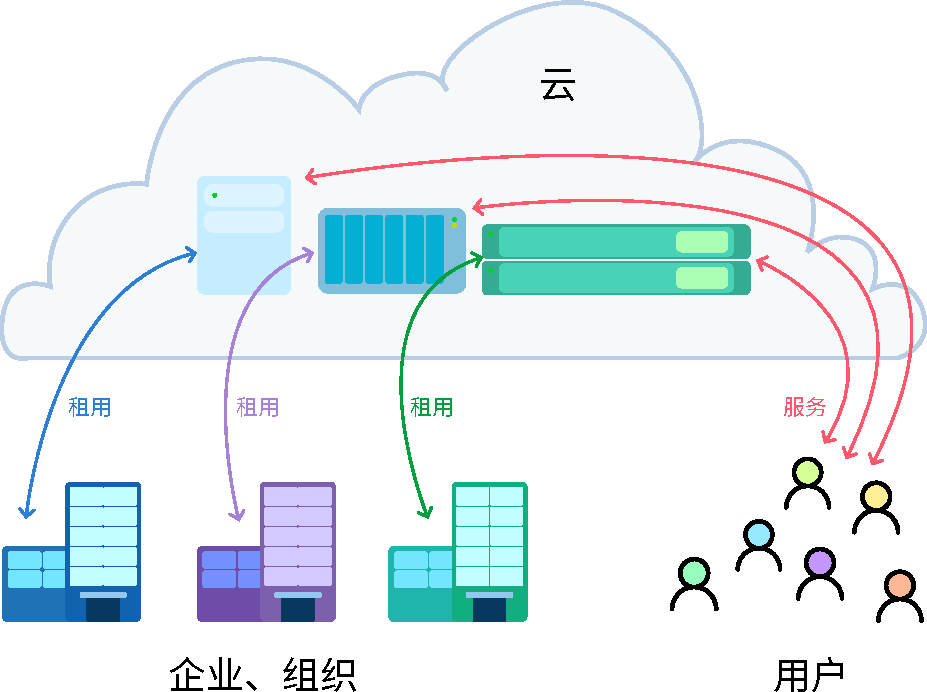
\includegraphics[width=.85\textwidth]{assets/surpass/The_Cloud.pdf}
  \caption{「云」}
  \label{fig:The_Cloud}
\end{figure}

「没错。从无数苦痛中蜕变,『云计算』的时代,就此拉开序幕……」

\section{第二幕·曙光 2014·「云」的计算与「物」的联网}

21 世纪的第一个十年已经过去,中国也继续驶向产业转型升级的快车道,整体工业水平也随之不断提高。在这样的大趋势下,生产设备的零件精度更加是重中之重。

她是本地一家轴承厂的工程师与质量主管,这家工厂主要生产高精度滚动轴承及其附属配件。得益于优良的精度与稳定性,外加当地成体系的产业链,轴承厂的销量颇丰,效益不错。但最近,售后部门频频接到客户投诉,不是轴承游隙有问题,导致运转不稳定;就是公差不满足,装都装不上去。售后把投诉统计放到她眼前:「你是管产品质量的,看看这是怎么一回事?」

「我立马排查。」她如是回复。人员、机器、原料、方法、环境,五大方面,她一个个排查,最终确定是生产设备老化、质检工疏忽大意导致了这些次品的流出。但她想得更远:不能总是等到投诉了才来亡羊补牢,必须将这些次品隐患消除在工厂内。

她冥思苦想、四处寻找灵感。一次行业内先进技术交流会上,台上的人正在介绍「工业物联网」。她立刻看向台上:「什么\CJKunderline{物联网}?不是\CJKunderline{互联网}吗?」然而大屏幕上明明白白地写着「物联网」。随后,她看到了管理部门电脑上琳琅满目的信息,从设备的温度、振动、损耗情况,到产品的在线检测图像、性能测试数据,再到自动分析出的可能存在的风险……就像阿基米德灵光一闪突然跑到大街上喊「尤里卡!」一样,她也万分激动,因为她找到了自己日思夜想的方案。

回到公司,她立马在会议上提出了自己的质量整改方案,得到了领导的高度认可。于是,她与当地院校合作,在工厂内引入了一套物联网方案。为存储与分析数据,他们在一家云计算平台租了一台「云服务器」。在平台上,他们可以自己配置服务器的 CPU、内存、硬盘等参数,而下单得到的,则是远处一台服务器的「完整使用权限」。他们只要用就行了,无需关心网络与维护这些琐事。在服务器上,他们安装了整套用于数据收集与处理的软件。

车间中,各种数控机床装上了数据收集、远程控制软件,将数据传到云服务器上。而那些没有数控的老旧设备,则装上了各种传感器来尽可能收集监测数据,同样传到云端。这些数据经云服务器处理,呈现在质量管理部的电脑上,她和同事们,在算法的帮助下,能及早发现问题、排除隐患,将次品扼杀在摇篮中。

这套系统投入使用后,次品率大幅降低,轴承的精度也比原来更好。当地政府甚至将这套系统作为「智能制造」标兵项目宣传。然而,鲜花与掌声中,她也听到了一些犯难的声音:「这套系统,跟大学合作的,要花不少钱呢!」「确实,而且还要有技术人才,我们这种小厂哪里担负得起啊……」

她很高兴,自己的决策成为了优秀的榜样;她也有些忧伤,这套系统需要先进的技术与大量资金支持,复制并不容易。虽然智能制造的「未来工厂」只是曙光初现,但她坚信:未来的工厂一定是万物连接到云端的,用数据让每一道工序都趋近完美。

\section{幕间·二}

「我感觉『智能工厂』这个东西是最近几年才开始大肆宣传应用的,没想到这么早就有先例了吗?」Windy 小啜一口饮料。

「虽然似乎是这样,但是一项技术从开发到推广肯定是需要一些时间的。早在 2006 年,美国的亚马逊就推出了一款名叫『弹性云计算』的服务,他们叫『Elastic Compute Cloud』,简称『EC2』。借助这个 EC2,用户就能租到开箱即用的服务器,非常方便。」

「你这『开箱即用』,是不是就是刚才你讲的那种『从平台上就能方便配置的云服务器』?」

「就是这种。服务器实际上在亚马逊的机房内,用户可以拿它建网站、运行服务、分析数据……各种事情都可以,而不需要——当然也没法——关注电费、维护等琐事,只要根据用量或者使用时长付租金就行了。」

「你这么说,看来亚马逊的地盘蛮大的,能放下这么多服务器租给用户。」

「这就不太可能了。全球这么多用户,每人一台机子那还得了,辟一个公园都放不下吧。」

「那怎么办?」

「虚拟化。云服务器不是可以根据用户需求组织配置吗?若真为这么多不同组合分派不同硬件,显然更不现实。而\regcolor{利用虚拟化技术,人们就可以在一台电脑上,用软件模拟出多台『虚拟机』},这些虚拟机之间就像独立的电脑一样,彼此感知不到对方,但可以灵活配置、独立开关机,甚至可以随意创建或删除。」Hans 也喝了一口饮料。

\begin{figure}[htb!]
  \centering
  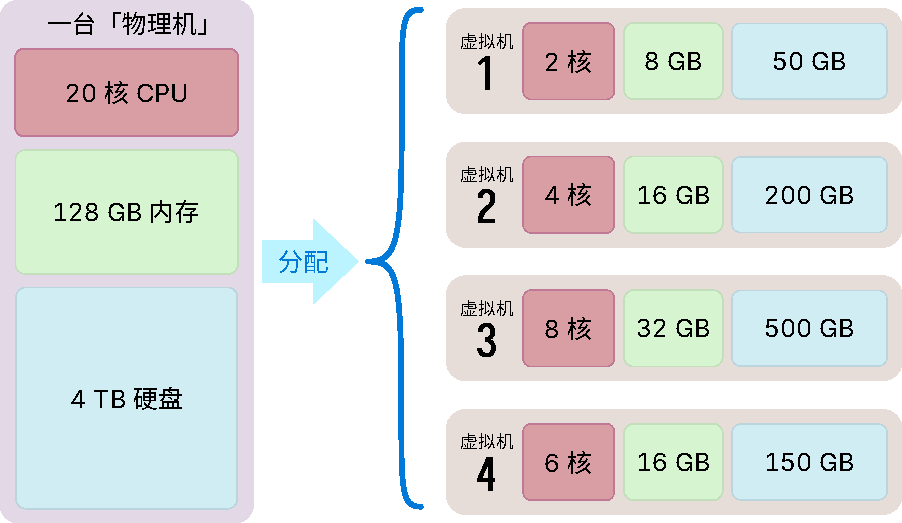
\includegraphics[width=.7\textwidth]{assets/surpass/VMs.pdf}
  \caption{虚拟机}
  \label{fig:VMs}
\end{figure}

「哦~这么一来,亚马逊机房的服务器就通过虚拟化,分出一大堆云服务器,而用户得到的其实是这些分出来的虚拟机。既方便厂商,又方便用户,真是双赢的局面。」

「的确,所以后来有许多厂商都开始推出这样的云服务器,比如国外的微软、谷歌,国内的阿里、盛大、腾讯等等。这些公司各自在定价什么的方面还有不同,人们还给它们起了一堆外号呢。」

「啊?还有这事?」

「是的,你可以上网去搜搜。总之,差不多 2010 年,云计算围绕云服务器,开始快速发展。这是一种『算力集中化』——计算能力集中到了服务商的手中,整合资源,按需分配。」

「但是要撑起『她』工厂里的智能系统,光有服务器不够啊,还有设备上的那一堆数据采集装置呢。」

「这就是『物联网』的力量了。『云』是中心,那么『物』就是边缘。\regcolor{物联网的目标,就是让万物都成为『边缘』,接入网络。}」Hans 准备终结盘里的牛排。

\begin{figure}[htb!]
  \centering
  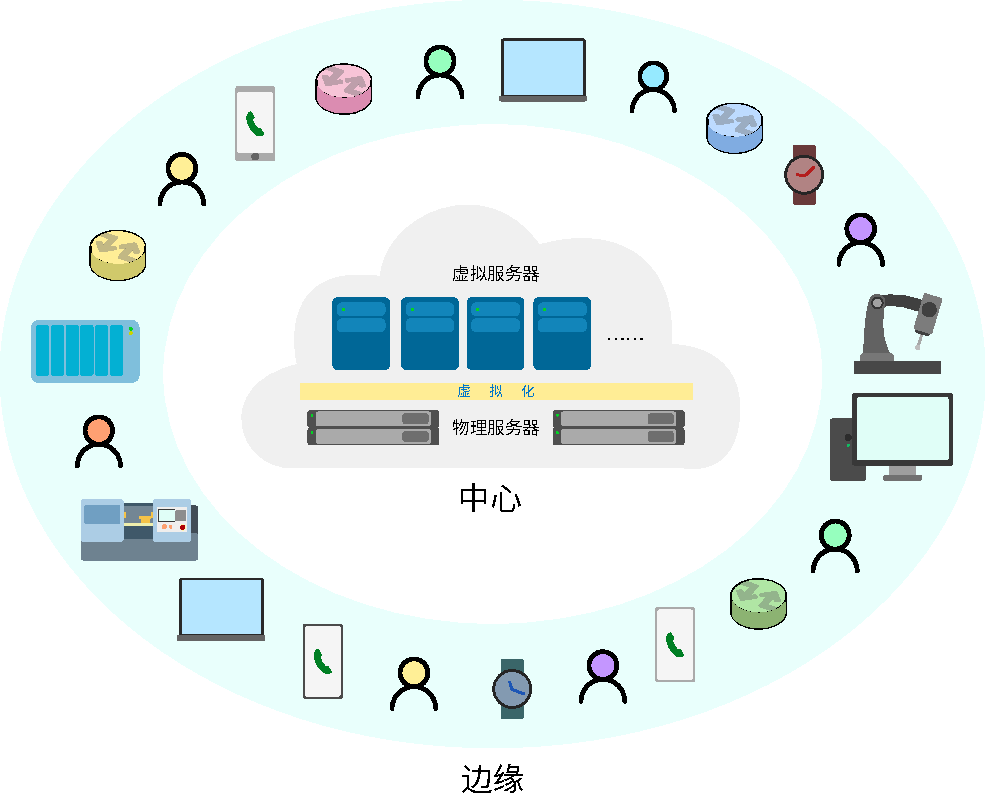
\includegraphics[width=.8\textwidth]{assets/surpass/Centre_and_edge.pdf}
  \caption{中心和边缘}
  \label{fig:Centre_and_edge}
\end{figure}

「所以,借助物联网的力量,工厂里那些改装过的设备也变成了网络的一部分。这样一来,机器工作过程中的实时状态都能通过网络传到云服务器进行分析,再向管理者的电脑发送结果。那么,整个车间的生产情况、存在的隐患、各种机床的实时工况,都能为管理者所知。」

「不仅如此,在生产设备上还可以加装一种超级小的电脑,叫做『\regcolor{嵌入式计算机}』。只要这么大一块电路板,上面就能塞进处理器、内存和类似硬盘的部件。显然它们性能不强,不过也足够它们自行控制这些机器了——或者从云端接收管理者的指令,让远在另一端的管理者也能控制这些设备。」Hans 用手指比划着银行卡一般大的长方形,说道。

「这是不是一种『运筹帷幄之中,操纵千里之外』?」Windy 消灭了最后一块炸鱼。

「依靠云服务器这座『桥梁』,还真是这样。」Hans 起身,「吃饱了,再去别的地方转转吧。」

二人移步图书馆,流线形的外观让这栋建筑看起来更像「知识的海洋」。Hans 再一次当起了导游:「这是我们的图书馆,但同时也对市民开放,大家都可以来这里办证借书。」

「高级。『好的大学,没有围墙。』」

拾级而上,穿行在一排排书架间,Hans 面露喜色,抽出一本《新手学电脑一本通(Windows 7 版)》:「你看,这是我们的竞品。」

Windy 翻着书,也跟着乐:「可这都是老久之前的书了,咱们可是与时俱进的!」\footnote{图书馆禁止大声喧哗哦!即便是感叹,也只在细若游丝的声音上提高一点而已。}

「别说,我们的《你缺计课》也是依托云服务的。现在可是 20 年代了,时代变了,生活也变了。」

\section{第三幕·绽放 2024·授人以渔}

「你不觉得,我们身边有同龄人连电脑都不会用,这是很可悲的一件事吗?」

「的确,感觉这应该是个基本技能的。」

「我想写点东西……名字就致敬一下 MIT 的那个『Missing』,叫《你缺失的那门计算机课》,教一些电脑使用基本知识。」

「我觉得挺好的,值得一试。」

「一起写?」

「可。」

这场对话已是整整三年前的往事,但即便过去一千多天,这往事仍历历在目。临近 2024 的结尾,他回忆着三年前的往事,心中感慨万千。在当年鸡同鸭讲地给同学科普了电脑的基本操作后,他愤而提笔,立志写就一套面向当今「电脑小白」的电脑使用教程。他把这个想法告诉友人,便留下了上面的对话。那时的他们从未想到,看似一时兴起的决定能够一直坚持到现在。

回到三年前。说干就干,二人很快开始构思、动笔,写下一篇篇文章。他们迫不及待地想把自己的作品分享给大家,尤其是那些需要帮助的人。但是想法很热切,现实却有麻烦,怎样既能方便快捷地协作编写,又能轻松地把作品分享出去呢?他们找到了一款「在线文档」,两个需求一次满足!得益于「在线」特性,所有内容都安全地存在云端,随时随地任何设备都能查看。短短几个月,二人写下了六万多字。

看起来一切稳中向好,但是在线文档的问题也逐渐凸显,他们想要推广作品却受到了一些掣肘——分享链接不利于推广,看起来像什么奇怪小网站似的。于是,他们想建立自己的网站,并把作品搬上去。这次,他们选择了一个能免费托管代码与文档的云平台。这款平台还提供了一键从文档生成网站的服务,只需简单配置参数,就能搭出简洁美观又大方的网站。

但是免费平台终究有其限制:访问速度差强人意、存储空间相当有限。他们开始寻求更好的云服务器。云服务器市场经过了十几年的发展,低配的选项已接近「白菜价」,只要几百块一年,就能租一个足够网站运营起来的云服务器。他精挑细选,在一家国内的云计算平台租好了服务器。在搭建网站之余,他还利用富余的性能,搭建了一款知名游戏的服务器,与友人一同愉快游玩。

这样一来,他们的作品能够为更多的人看到,也能够帮到更多人。他们喜悦于自己的作品能传播开来,授人以渔;同样感慨于自己一路上能持之以恒、始终如一。他们更加相信,用心写下的作品能不断壮大、越来越好,也希望需要它的人都能获得这份知识。

\section{幕间·三}

两人缓步走出图书馆。Windy 回望流线形的「知识之海」,感叹:「知识使人类进步,科技能改变生活。」

「的确如此。曾经,云计算服务商主要是提供各种云服务器,客户大多都是有一定规模的企业与组织,这种模式叫「\regcolor{基础设施即服务}」,简称 IaaS。现在,云计算则演化出「\regcolor{平台即服务}」和「\regcolor{软件即服务}」的新形态,分别简称 PaaS 和 SaaS——\regcolor{用户不用再买完整的服务器,也无需学习服务器的配置和使用,而是选购云计算厂商提供的某一项具体功能或服务。}

「那我们常用的各种『网盘』,还有当初我们用的在线文档,看来都是这种云计算模式了?」

「对。相比 IaaS 的『卖算力』,PaaS 和 SaaS 就是在『卖应用』。除了云盘和在线文档以外,我们当初用的『从文档生成网站』的服务也是一个例子,我们不需要考虑具体如何搭建网站,只要配置一下,就能直接用了。」

\begin{table}[htb!]
  \centering
  \caption{三种云服务模式的对比}
  \label{tab:3-types-of-cloud-service}
  \begin{tblr}{
    colspec = XX[4]X[4],
    % hline{2} = {2-Z}{solid,white},
    % vline{2} = {2-Z}{solid,white},
    % hline{2-Y} = {1}{solid,white},
    % vline{2-Y} = {1}{solid,white},
    % hline{3-Y} = {2-Z}{solid,missing},
    % vline{3-Y} = {2-Z}{solid,missing},
    % hline{1,Z} = {solid,missing},
    % vline{1,Z} = {solid,missing},
    row{1}      = {font=\bfseries, bg=missing, fg=white},
    column{1}   = {font=\bfseries, bg=missing, fg=white},
    cells       = {halign=c, valign=m},
    cell{1}{1}  = {bg=MissingSkyBlue, fg=missing},
  }
    \toprule
    & IaaS & PaaS 和 SaaS \\
    产品种类 & {单一\\基础计算资源(如云服务器)} & {多样\\各种应用和平台} \\
    定价 & {较高\\按租用时长或用量计费} & {较低\\通常按使用量或用户数计费} \\
    易用性 & {低\\使用者需掌握服务器运维知识,需手动搭建各种服务} & {高\\容易上手,只需少量,甚至无需专业知识} \\
    受众 & 企业、组织、专业人士 & 企业、组织、专业人士、大众 \\
    \bottomrule
  \end{tblr}
\end{table}

「我又想起一种很新的云服务:『云电脑』『云游戏』什么的。照你的说法,它们应该混合了这两大类模式:硬件层面上,它们算一种 IaaS,既然云计算服务商能虚拟出一堆好用的服务器,那虚拟出一台普通电脑,或者游戏电脑,也不是什么难事;不过从易用性角度看,用户能很轻松地购买、使用,甚至都不用自己安装软件,又更像 SaaS。」

「没错!这也是『算力集中化』的进一步体现。在云游戏和云电脑普及开来后,高性能的算力集中到了云计算服务商那里。之前,玩家需要自己购买高配置的 CPU、显卡等硬件,现在就只需要花点小钱租个云电脑就行了。」

「不过说到底,这么些服务还是基于网络的,先不说没网就用不了,云盘还需要高速传输才好用,而云电脑或者云游戏,超低延迟是硬指标。好在,更先进的高速 Wi-Fi 标准,以及 5G 的全面普及,让高速高质低价格的网络成为了可能。」

「我们平常用的网盘还算好,有的虽然慢,至少你的资料是一分不少。但是有的云盘服务,用着用着,你的文件可能就不见了,本来生态又封闭,想找回文件更是难上加难、雪上加霜。」Hans 摇着头,对不知哪家云服务厂商如是评价。

「不会吧,这样的厂商还有人用?」

「谁知道呢,」Hans 摊了摊手,「总之,我们学校就差不多逛完了,还是挺小的吧。」

「确实,但『麻雀虽小,五脏俱全』。剩下还有时间,之后去哪玩呢?」Windy 人生地不熟。

「去附近的海湾公园看看吧。」

Windy 想起什么,戳了几下自己的智能手表:「说起物联网,我觉得如今物联网也不是工厂里才能用上的玩意了。比如说我家里就有一些智能家具,能直接连到我家的 Wi-Fi,我在手表上也能远程控制它们。」

「好家伙,给我看看。」

「你看,点这里,门就可以反锁或者解除反锁,还能查看最近的开门记录;点这个灯,就可以开灯或者关灯,还能调亮度。还有别的什么冰箱啊路由器什么的,都可以统一控制……」

\begin{figure}[htb!]
  \centering
  
\includegraphics[width=.8\textwidth]{assets/surpass/Smart_watch.pdf}
  \caption{Windy 的智能手表}
  \label{fig:Smart_watch}
\end{figure}

「哈哈哈哈哈哈哈哈哈……」

「呃,嗯,对,我这里调整了什么,家里人的手机上也会有显示。这就是物联网的魅力啊!」Windy 强作镇定。

「确实,你说得太——对——了。」Hans 打趣。

「反正,这些智能家居,在嵌入式计算机的加持下,能够联网、远控,据说更高级的还能分析数据,让生活变得更加方便。我这手表还有好多健康监测功能,像心率啊睡眠啊之类的都会长期记录。从工业到民用,物联网的边界还在不断拓展。」

Hans 的学校到海湾公园不算遥远,也就几站路。从地铁站出来,放眼望去,潮涨潮落拍打岸堤、绿树青草触手可及,还有人、人,以及更多的人,在公园游走。海风轻拂,为繁忙的公园带来了一些自然的享受。

「你们这中秋真热闹啊。」Windy 看着满大街的人。

\begin{figure}[htb!]
  \centering
  
\includegraphics[width=.7\textwidth]{assets/surpass/The_seaside_park.jpg}
  \caption{海湾公园}
  \label{fig:The_seaside_park}
\end{figure}

「过节都这样,大家都来看看海。」Hans 倒觉得稀松平常。

漫步在海岸线上,远望城市里林立的高楼,Hans 感叹:「是啊,十年前,物联网还是工厂中最先进的技术;十年后,在地球上任何一个有网络的地方,我们都能用手机——甚至手表——控制家中的一切。这个过程中,控制的方式、设备的种类都在变化,不变的是云计算这座『桥梁』。乘着云计算的东风,更多的厂商能够入局物联网,在水中激起一片又一片涟漪,促进着市场的良性循环;市场的不断扩大,又在影响物联网与云计算的不断演进。不远的将来,或许会是沧海桑田……」

\section{第四幕·幻想 20?4·「我们」的世界}

清晨,随着一阵轻音乐,遮光窗帘自动缓缓滑开,让晨光洒入房间。她随着乐声醒来,拿起手机,关闭闹铃,「您昨晚睡眠质量良好」。起床,洗漱,走进厨房,拿出自动烹饪机器刚刚准备好的早餐,「根据您最近的健康状况,早餐特别添加富含维生素 D 的金枪鱼肉」。手机上又弹出通知:「您的牛奶已送达,请及时拿取。」她转头,看见阳台上的新鲜牛奶,伴随着逐渐远去的无人机旋翼声,她取回牛奶,开始享受早餐。

在城市另一侧,他的一天从公司的线上早会开始。他轻触墙上中控台的「模式」按钮,切换至「专注模式」。空调转为低风,降低噪音;墙面换成米色,朴素舒适;麦克风自动降噪,屏蔽环境音:他的家为会议做好了一切准备。此刻,来自全国各地的员工通过互联网在空中相遇,却如同近在眼前,共同商讨本周的建设计划。会议圆满结束,系统自动生成了一份完整的会议纪要,发送到每个人的手机上。

你正在前往公司的路上,城市的风光尽收眼底:道路中,一辆辆自动驾驶汽车飞驰而过;高处,无数的无人机穿梭于天空,向各地运送包裹;路边,城市清洁车正在自动回收垃圾,清扫街道;各处的绿化带里,草木在自动监测系统的加持下保持着最佳活力;街头巷尾的商铺,正充满朝气地开始一天的营业。你又看了一下中控屏上的路程信息,还有 20 分钟,不如小憩一会。

她前往城郊的生态实验站,这里是她的工作地点,也是全国生态数据采集系统庞大网络的一个节点。她站在山巅,脚下的绿水青山令她心旷神怡,而手中的平板显示着这片山林的另一面:林中隐秘的摄像头观测着野生动物的活动状态与范围、鸟群的迁徙路线与飞行轨迹、植被的生长情况与分布,遍布的传感器探测着这片大地的地质变化、水体质量、空气温湿度与质量。此时,平板上传来同事的消息:「昨天我们的机器人在西边山谷 240 m 深处采集到的珍稀植物样本已完好抵达最近的生物实验室,正在进行进一步研究。」

结束早会,他把家中切换为平时的工作模式,和煦的阳光令他舒适无比。他坐在电脑前,时不时操作一下键盘。与此同时,远处的工地上,形态各异的机器人热火朝天地忙碌着,巨大的 3D 打印机开始打印大楼的框架,一座高楼正这样拔地而起。工地上的一切都在云端的控制之下稳步前行,而他的工作,便是在电脑上通过云端统筹调度。上周,公司刚刚完成一个项目的验收,新建的大楼或许很快就有客户入驻。

一天的时光总是如此有限,黄昏已临,夜幕将至,城市的灯光渐次亮起。我望着窗外,回想着这座城市的一天,虽忙碌,却仍旧幸福。偶尔想自己下厨制作晚饭,也只需拿起手机订购食材,就能很快收到。星空璀璨,明天的太阳一定更好。

\section{尾声}

夕阳将天空染成黄色,为云朵镶上橙色,水波金光粼粼,闪亮而耀眼。二人散步许久,在长椅上歇息。Windy 说:「我们实在难以想象未来的生活会是如何,毕竟人无法想象出超越自己认知的事物,但有件事是肯定的——生活一定会更加美好。」

\begin{figure}[htb!]
  \centering
  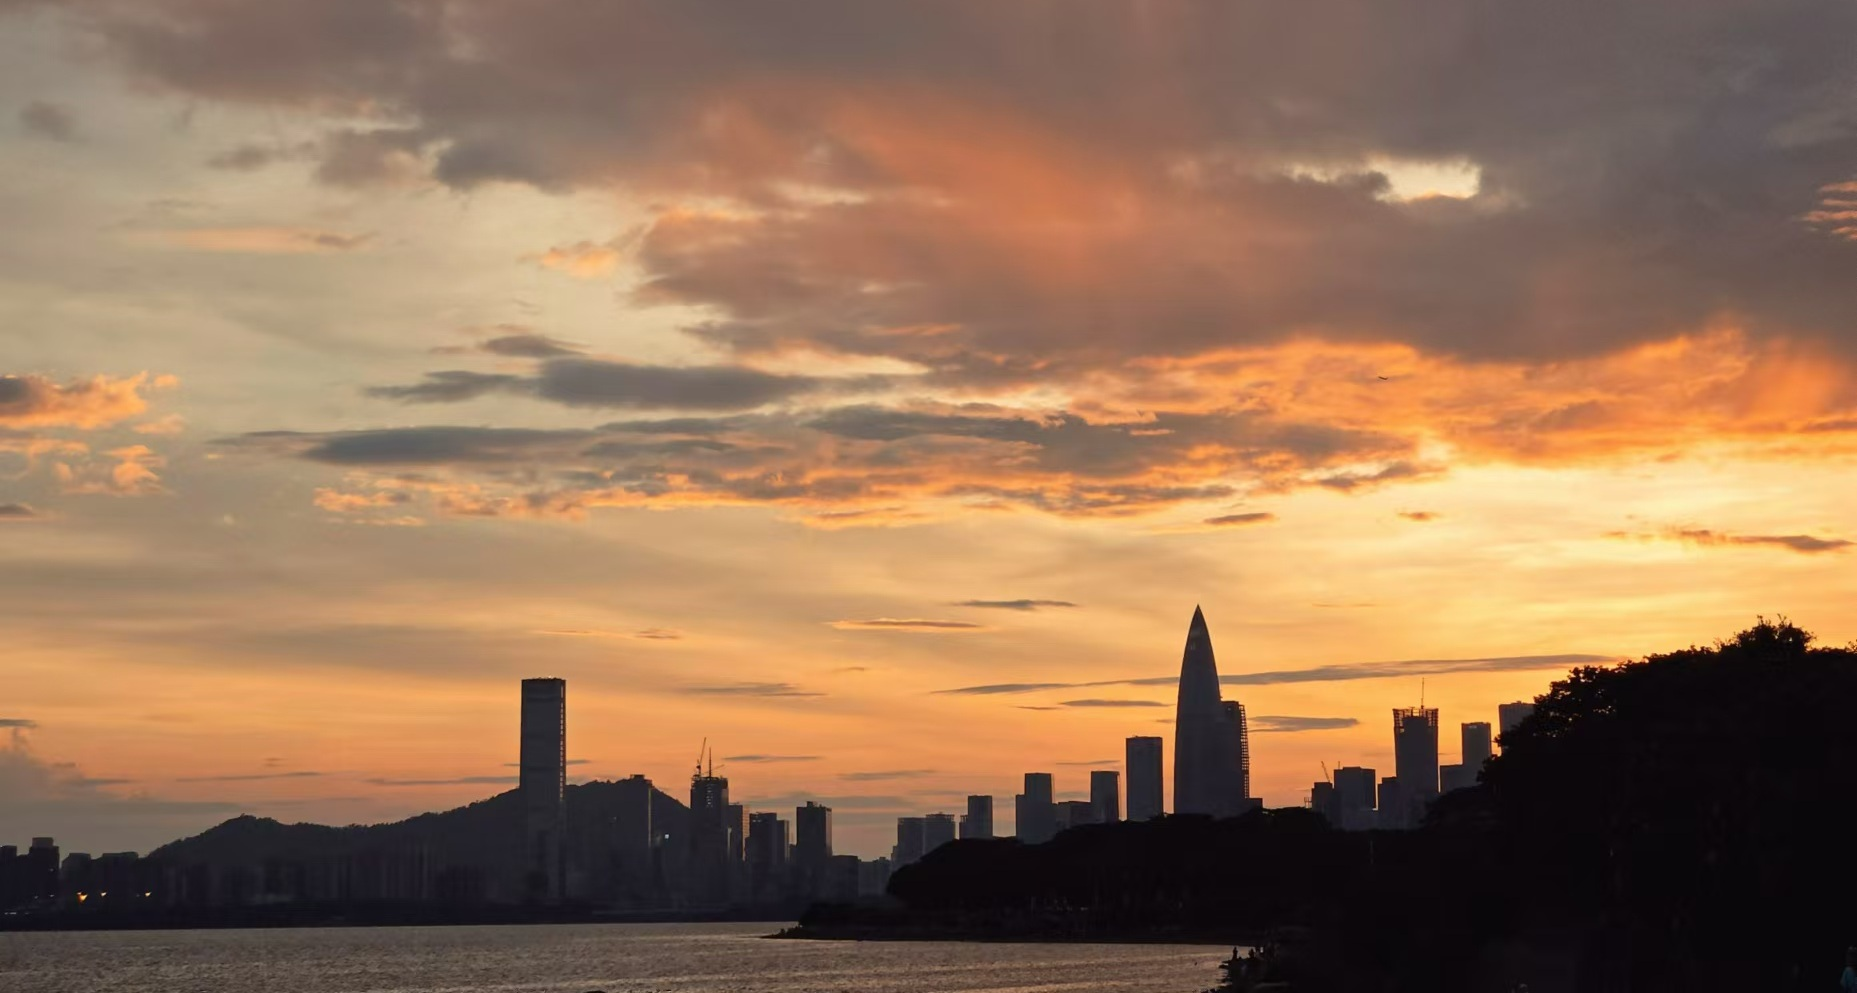
\includegraphics[width=.7\textwidth]{assets/surpass/The_dusk.jpg}
  \caption{夕阳}
  \label{fig:The_dusk}
\end{figure}

Hans 笑言:「虽然是这样,但幻想将来不也是一件美好的事情吗?在如今科技的浪潮中,\hyperref[cha:bring-intelligence-to-machines]{\CJKunderwave{人工智能}}、\hyperref[cha:introduction-to-cryptology]{\CJKunderwave{密码学与网络安全}}、\hyperref[cha:program-and-arch]{\CJKunderwave{程序语言与计算技术}},以及\hyperref[cha:cloud-computing-and-iot]{\CJKunderwave{云计算和物联网}},正撼动着各自原本封闭的孤岛,交融成为一块整体的大陆。它们的互相成就,不仅拓展了技术的边界,更在人类生活的方方面面开启了新篇章。」

「是啊,云计算为人工智能提供高性能算力与海量存储空间,AI 模型训练与推理变得更加高效普惠;物联网为 AI 提供无数『感知之眼』,通过这些物联网设备,无论是家庭、城市、工厂,还是生态、自然,AI 都能实时获取数据,持续优化自身。他们的交融,正在推动我们从数字时代进发到智能时代,从感受世界到做出决策的每一环都简单高效。」

「照这样的趋势,这种协同交融应该会促进技术的复杂应用。比如说智能驾驶,车辆上的边缘设备能够实时处理车辆周围的环境感知,而较复杂的路径规划等工作则交给云端 AI 完成。在医疗、农业还有其他领域也是类似,边缘设备提供及时响应,云端系统为长期优化提供支持,二者互相补充,重新定义技术的效率和边界,帮助人们快速做出更优的决策。」

「这样的话,肯定会包含一些安全隐患吧?比如,要是让黑客攻击了路上的车,把我的车偷了,甚至是远程驾驶它去撞人怎么办?还比如我这手表,它会不会偷偷用我的生理数据去干些什么不道德的事?」

「没错,即便是现在,数据隐私和网络攻击都不时成为社会热点,但密码学与网络安全技术正在为隐私保驾护航。在传统的加密、哈希、签名和证书技术的基础上,人们又研究出了用于隐私计算的安全多方协议,更有『零知识证明』和『联邦学习』等等新兴技术。在云与物联的世界中,这些新兴的保护手段不仅在云端构筑了坚不可摧的防线,更延伸到了每一台物联网设备、每一个边缘节点,技术生态在透明与隐私之间终会找到一个平衡。」

「知识使人类进步,科技能改变生活。在技术进步越来越快的现在,在『为人类服务』的宗旨下,我们的工作、我们的生活、我们的创造,终将享受到技术进步带来的便利。人类的社会更将因此迈向更高效、可持续、命运共同、和谐共生的未来。」

似乎沉浸在思维之海中,二人望着天空,几时一言不发。

「时候不早了,我应该也要回去了。」Windy 起身,率先打破沉默。

「走吧,去地铁站。」Hans 也起身,拍了拍身上的尘土。

站台两侧,同属一条线路的两趟列车相背而行,驶向各自的远方。

天空中,繁星依旧璀璨而绚烂,正如这个世界的未来。

\practice

\begin{enumerate}
  \item 请用自己的语言回答「什么是云计算」。
  \item 请用自己的语言回答「什么是物联网」。
  \item 「互联网+」是近些年非常火热的一个概念,它指的是「互联网」与传统领域的结合,例如「互联网+工业」「互联网+医疗」。请上网搜索一个「互联网+」的特定领域,然后试着分析云计算和物联网在其中的应用。
  \item 至此,《你缺计课》的正文内容已经全部结束,分享一下你的感想和体会。如果愿意,你可以发送到我们的邮箱 \href{mailto:missing@criwits.top}{\texttt{missing@criwits.top}}。
\end{enumerate}